% %%%%%%%%%%%%%%%%%%%%%%%%%%%%%%%%%%%%%%%%%%%%%%%%%%%%%%%%%%%%%%%%%%%%%
% Section N
% %%%%%%%%%%%%%%%%%%%%%%%%%%%%%%%%%%%%%%%%%%%%%%%%%%%%%%%%%%%%%%%%%%%%%

\section{An Other Section}
\label{sec:section_n}

\subsection{Example of Figures}

\subsubsection{Position of the Figure}

\lipsum[1-2]

%% Use vectorized files, such as PDF, as much as possible for better quality

%% Figure at the top of the page by default, or using [t]
\begin{figure} %[t]
    \centering
    %% width=0.2\linewidth is scaling the image based on the current width
    %% of the environment.
    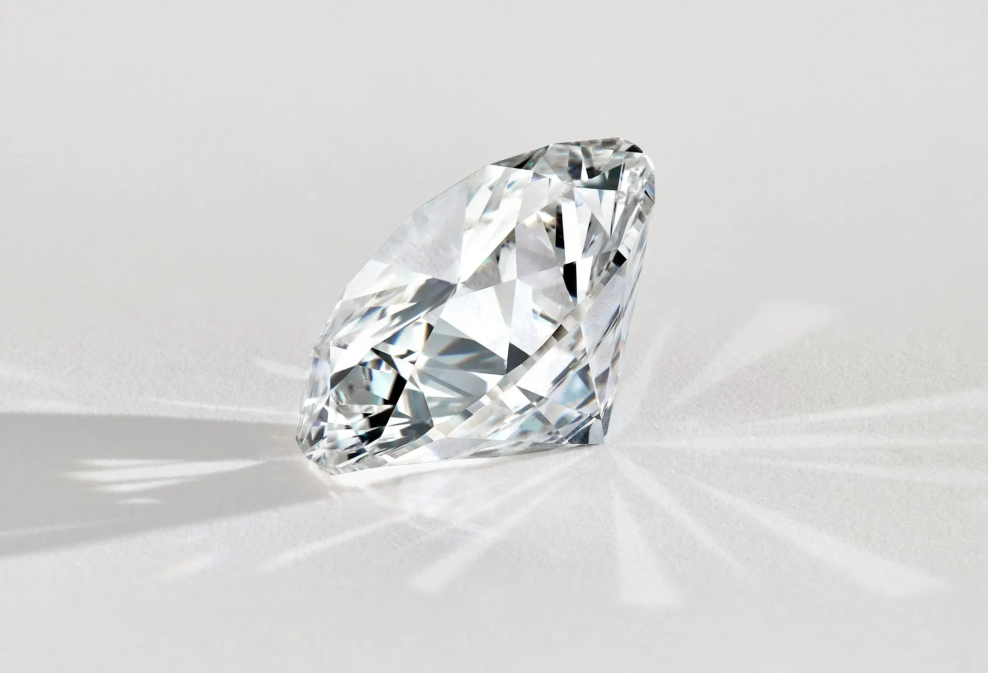
\includegraphics[width=0.2\linewidth]{Chapter_X/Figures/PDF/diamon1.pdf}
    \caption{Default (\textit{t}): Top of the page}
    \label{fig:ex1}
\end{figure}

%% Figure in the text, using [h]
\begin{figure}[h]
    \centering
    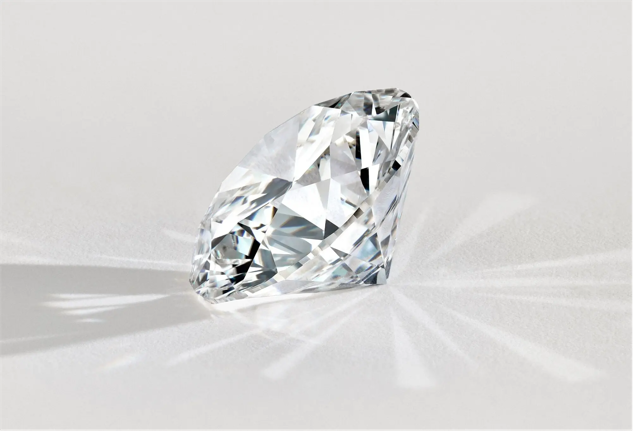
\includegraphics[width=0.2\linewidth]{Chapter_X/Figures/PDF/diamon1.png}
    \caption{With \textit{h}: Between the paragraphs}
    \label{fig:ex2}
\end{figure}

%% Figure at the bottom of the page, using [b]
\begin{figure}[b]
    \centering
    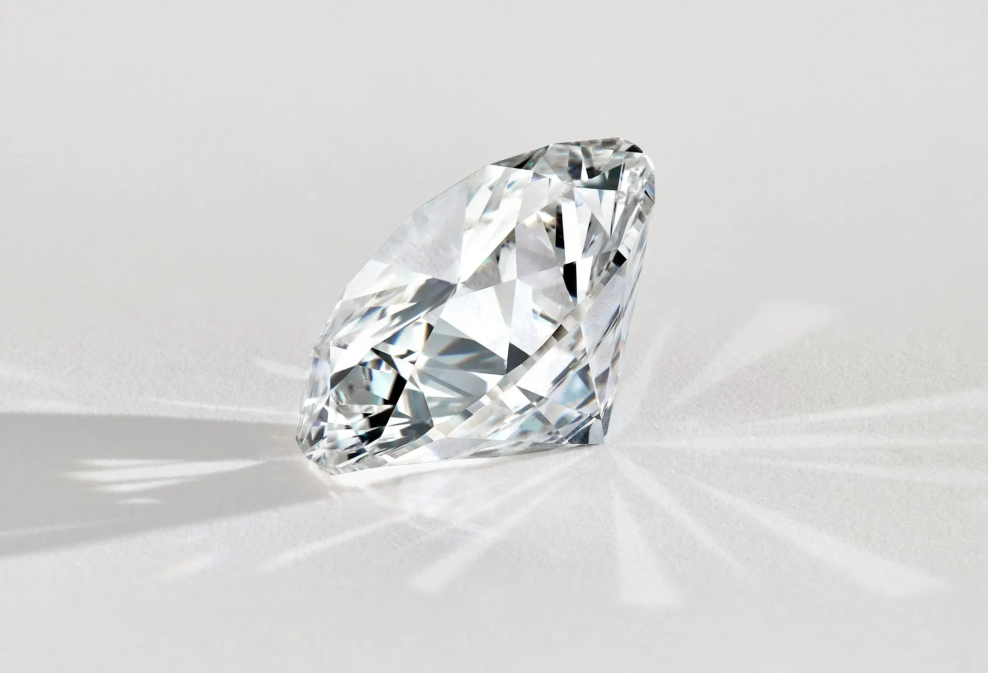
\includegraphics[width=0.2\linewidth]{Chapter_X/Figures/PDF/diamon1.pdf}
    \caption{With \textit{b}: Bottom of the page}
    \label{fig:ex3}
\end{figure}

%% You can use any combination, such as [htbp] which is commonly used, to allow
%% latex to choose the best one, while respecting the order of priority.
%% (p for page, the figure is taking an entire page, potentially with other figures)

\lipsum[3]

%% To reference a figure, use the \label{} + \ref{} commands
Reference to a figure: Figure~\ref{fig:ex1}.

\subsubsection{Subfigures}

References: Figure~\ref{fig:ex4}, Figure~\ref{fig:sub1}, Figure~\ref{fig:subsub1}.

\begin{figure}[h]
    \centering
    \begin{subfigure}{0.49\linewidth}
        \centering
        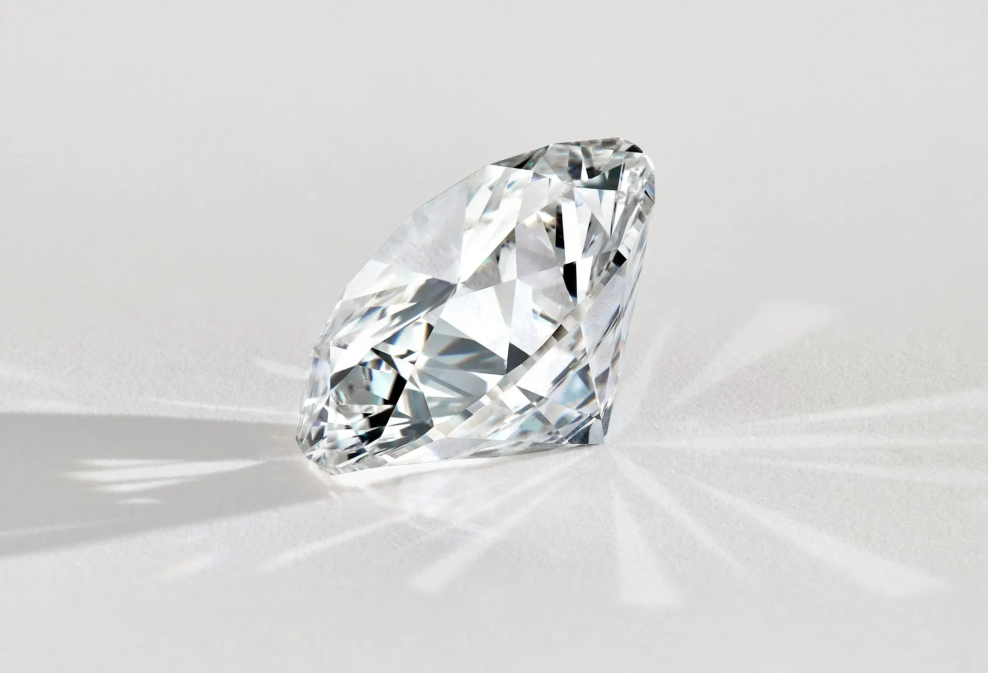
\includegraphics[width=1\linewidth]{Chapter_X/Figures/PDF/diamon1.pdf}
        \caption{A Figure}
        \label{fig:sub1}
    \end{subfigure}
    \hfill
    \begin{subfigure}{0.49\linewidth}
        \centering
        \setcounter{subsubfigure}{0}
        \begin{subsubfigure}{0.40\linewidth}
            \centering
            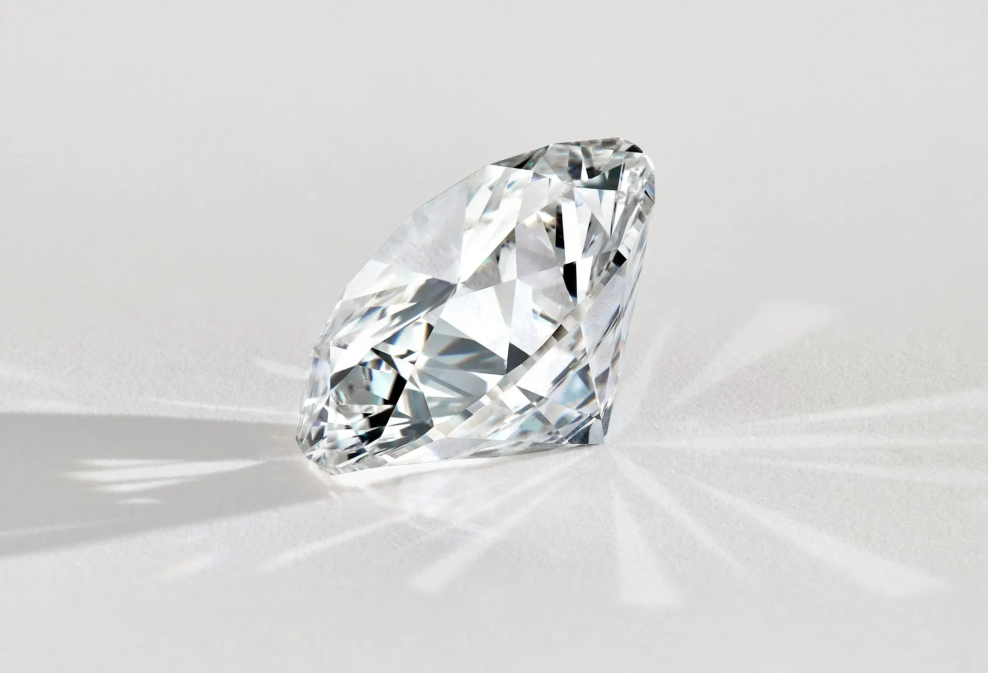
\includegraphics[width=1\linewidth]{Chapter_X/Figures/PDF/diamon1.pdf}
            \caption{A Figure}
            \label{fig:subsub1}
        \end{subsubfigure}
        % \hfill
        \begin{subsubfigure}{0.40\linewidth}
            \centering
            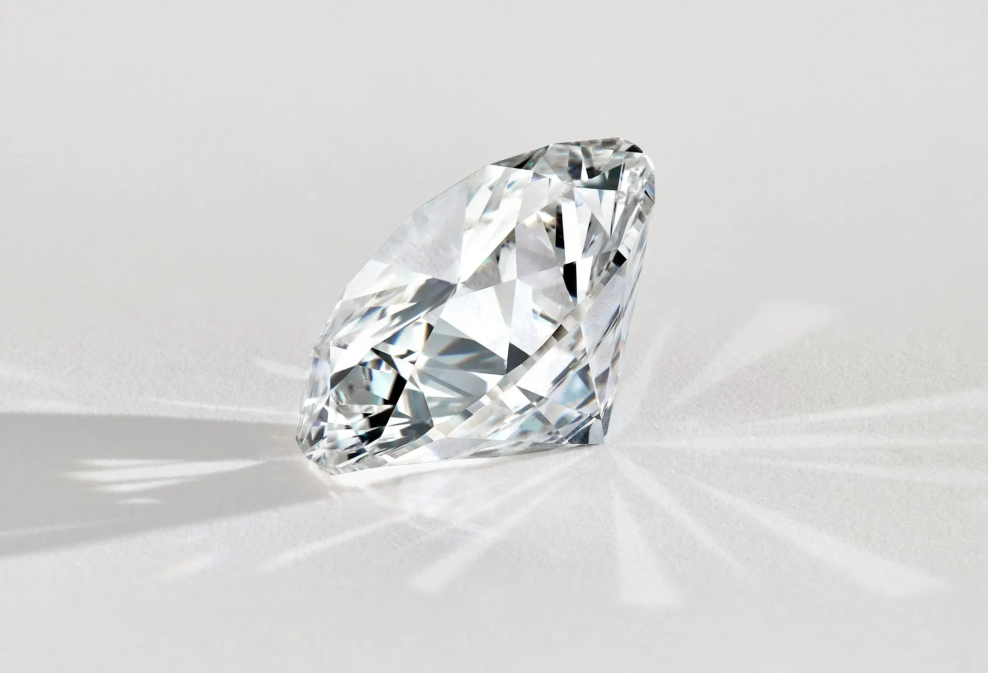
\includegraphics[width=1\linewidth]{Chapter_X/Figures/PDF/diamon1.pdf}
            \caption{A Figure}
            \label{fig:subsub2}
        \end{subsubfigure}
        \caption{A Subfigure with Subsubfigures}
        \label{fig:sub2}
    \end{subfigure}
    \caption{A Figure with Subfigures}
    \label{fig:ex4}
\end{figure}

\subsubsection{Two Figures Side by Side}

%% Use the minipage environment: it allows to define "boxes" of defined size
\begin{figure}[h]
    \centering
    \begin{minipage}{0.49\linewidth}
        \begin{figure}[H]
            \centering
            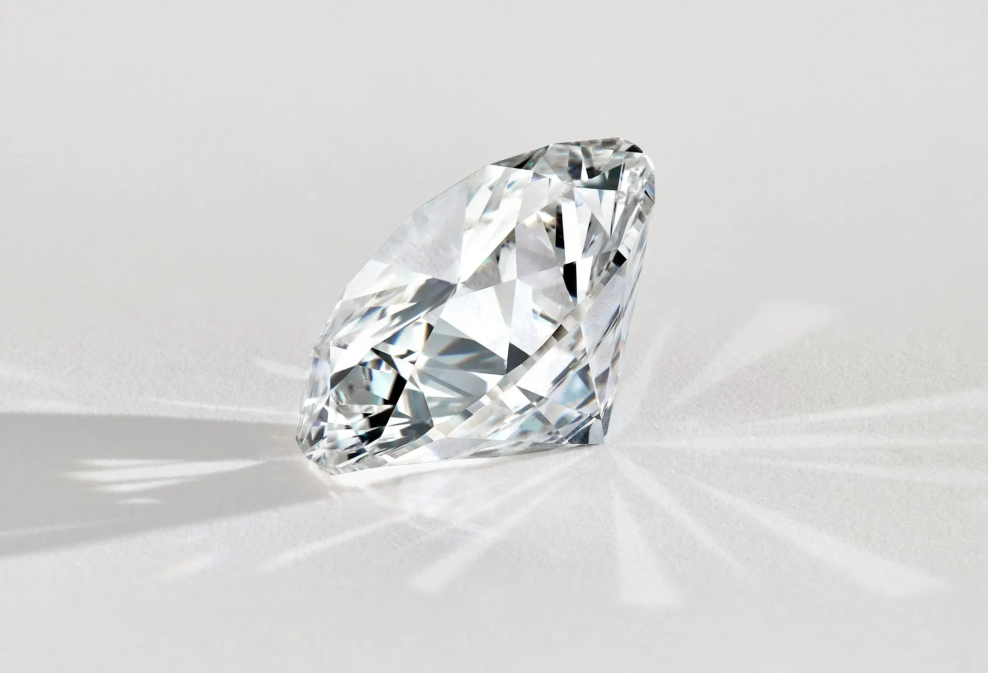
\includegraphics[width=1\linewidth]{Chapter_X/Figures/PDF/diamon1.pdf}
            \caption{A Figure}
            \label{fig:ex5}
        \end{figure}
    \end{minipage}
    \hfill
    \begin{minipage}{0.49\linewidth}
        \begin{figure}[H]
            \centering
            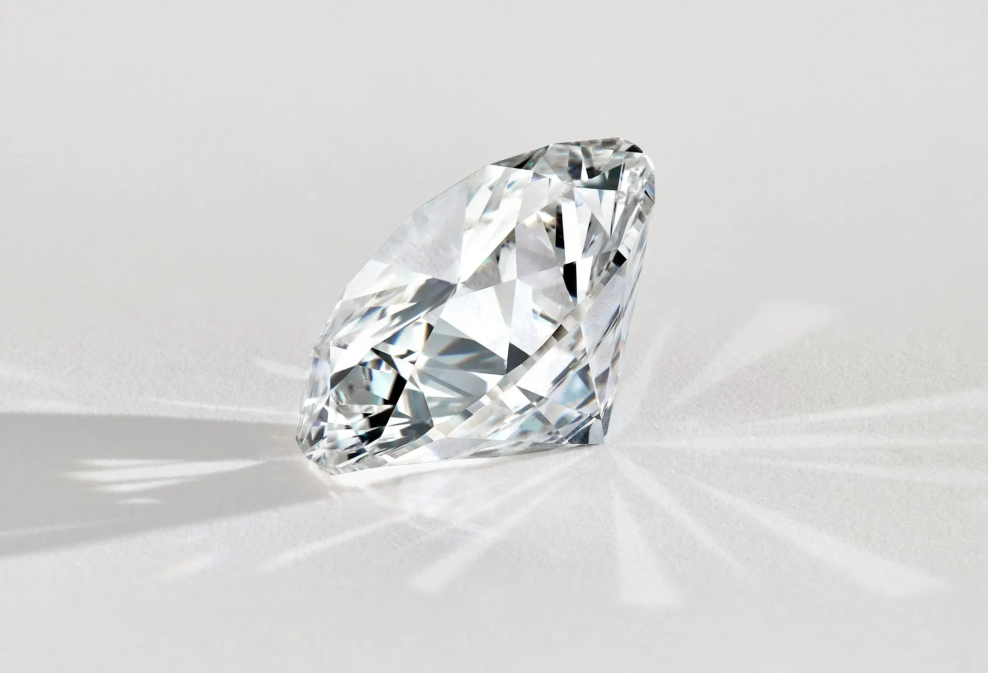
\includegraphics[width=1\linewidth]{Chapter_X/Figures/PDF/diamon1.pdf}
            \caption{A Figure}
            \label{fig:ex6}
        \end{figure}
    \end{minipage}
\end{figure}

\subsubsection{CEA Picture Library}

Some ``free-to-use'' pictures for CEA: \url{https://phototheque.intra.cea.fr/}

\subsection{Examples of Equations}

In line equations with \$$\centerdot$\$: $\forall a \in \mathbb{R}, a^1 = a$

%% \noindent to avoid the automatic indentation
\noindent Full line equation without environment with \$\$$\centerdot$\$\$:

$$\forall a \in \mathbb{R}, a^1 = a$$

\noindent Equation with environment, referenced as Equation~\ref{eq:ex1}:

\begin{equation}
    \label{eq:ex1}
    \forall a \in \mathbb{R}, a^1 = a
\end{equation}

Link for list of symbols in math mode: \url{https://www.cmor-faculty.rice.edu/~heinken/latex/symbols.pdf}

\subsection{Examples of Tables}

Reference to a table: Table~\ref{tab:ex1}.

\begin{table}[h] %% same placement parameters than figures
    \centering
    \begin{tabular}{c|cc}
        & \textbf{A} & \textbf{B} \\
        \hline
        \textbf{Oui} & 1 & 0 \\
        \textbf{Non} & 0 & 1
    \end{tabular}
    \caption{A Simple Table}
    \label{tab:ex1}
\end{table}

\begin{table}[h]
    \centering
    \begin{tabular}{|c||c|c|}
        \hhline{|-||-|-|}
        & \textbf{A} & \textbf{B} \\
        \hhline{=::==}
        \textbf{Oui} & 1 & 0 \\
        \hhline{|-||-|-|}
        \textbf{Non} & 0 & 1 \\
        \hhline{|-||-|-|}
    \end{tabular}
    \caption{A Simple Table Using \textit{hhline} Package}
    \label{tab:ex2}
\end{table}

\begin{table}[h]
    \centering
    \begin{tabular}{|c|c|c|c|}
        \hline
        & \multicolumn{2}{c|}{\textbf{A}} & \textbf{B} \\
        \hline
        \textbf{Oui} & 1 & 0 & 1 \\
        \hline
        \multirow{2}{*}{\textbf{Non}} & 0 & 1 & 1 \\
        \cline{2-4}
        & 1 & 1 & 0 \\
        \hline
    \end{tabular}
    \caption{A Simple Table Using \textit{multirow} and \textit{multicolumn}}
    \label{tab:ex3}
\end{table}

\begin{table}[H] %% H is forcing the position, else the two next tables are taking a new page
    \centering
    %% To use the >{...} options, and the m{...} configuration, the array package is needed
    %% The \arraybackslash command is needed to avoid errors in some cases
    \begin{tabular}{| >{\arraybackslash\raggedleft}p{3cm} | >{\arraybackslash\centering}m{3cm} | m{3cm} |}
        & \textbf{A} & \textbf{B} \\
        \hline
        \textbf{Oui} & 1 & 0 \\
        \textbf{Non} & 0 & 1
    \end{tabular}
    \caption{A Simple Table with Fixed Size Columns}
    \label{tab:ex4}
\end{table}

\begin{table}[H]
    \centering
    \caption{A Complex Table with Title Above}
    \label{tab:ex5}
    \begin{tabular}{|c||c||*{4}{c}|c|}
        \hhline{|-||-||----|-|}
        A1 & \multirow{2}{*}{B1} & \multicolumn{4}{c|}{\multirow{2}{*}{C1}} & \multirow{3}{*}[0ex]{\rotatebox{90}{D1......}} \\
        \hhline{|-||~||~~~~|~|}
        A2 & & & & & & \\
        \hhline{|-||-||----|~|}
        A3 & B2 & \multicolumn{3}{c|}{C2} & C3 & \\
        \hhline{:=::=::====:=:}
        1 & 2 & 3 & 4 & 5 & 6 & 7 \\
        \hhline{|-||-||----|~|}
        1 & 2 & 3 & 4 & 5 & 6 & 7 \\
        \hhline{|-||-||~|-|~~|~|}
        1 & 2 & 3 & \multicolumn{1}{|c|}{4} & 5 & 6 & 7 \\
        \hhline{|=||=====|=|}
        1 & 2 & 3 & 4 & 5 & 6 & 7 \\
        \hhline{|-||-||-----}
    \end{tabular}
\end{table}

A link to an online table generator: \url{https://www.tablesgenerator.com/}

%% \resizebox{\textwidth}{!}{} allow to resize the environment to the size of the page

%% if you want to start on a new page
\newpage

\subsection{Example of Algorithms}

Reference to algorithm: Algorithm~\ref{alg:ex1}

\begin{algorithm}[h]
    \caption{A Simple Algorithm with Comments}\label{alg:ex1}
    \KwIn{N}
    \For(\Comment*[f]{A comment}){$n \in [\![0, N[\![$}{
        $a \gets 0$\;
        \For{$i \in [\![0, 10[\![$}{
            $rand \gets \mathrm{Random}(0, 10)$\Comment*[r]{An other comment}
            $a \gets a + i \times rand$\;
        }
        \If{$a \leq 100$}{
            return $n$\;
        }
    }
\end{algorithm}

\subsection{Examples of Lists}

Example of list using the \textit{itemize} environment.
\begin{itemize}
    \item Something.
    \item An other thing.
\end{itemize}

\bigskip

\noindent Example of list using the \textit{enumerate} environment:
\begin{enumerate}
    \item something;
    \item an other thing.
\end{enumerate}

\subsection{Use of Glossary Entries}

Some text with the word \gls{op} and the word \gls{latex}, and then again \gls{op}, with its plural form \glspl{op}.

\bigskip

\noindent Some tests of glossary commands (see source code and \textit{Gloss\&Acro.tex}) with customized glossary entries:
\begin{itemize}
    \item \gls{gl1} \textit{(first call)} / \gls{gl1} / \Gls{gl1} / \glspl{gl1} / \Glspl{gl1}
    \item \glspl{gl2} \textit{(first call)} / \gls{gl2} / \Gls{gl2} / \glspl{gl2} / \Glspl{gl2}
    \item \Gls{gl3} \textit{(first call)} / \gls{gl3} / \Gls{gl3} / \glspl{gl3} / \Glspl{gl3}
    \item \Glspl{gl4} \textit{(first call)} / \gls{gl4} / \Gls{gl4} / \glspl{gl4} / \Glspl{gl4}
\end{itemize}

\bigskip

\noindent Some tests with customized acronym entries (see source code and \textit{Gloss\&Acro.tex}):
\begin{itemize}
    \item \gls{aptest1} \textit{(first call)} / \gls{aptest1} / \Gls{aptest1} / \glspl{aptest1} / \Glspl{aptest1}
    \item \glspl{aptest2} \textit{(first call)} / \gls{aptest2} / \Gls{aptest2} / \glspl{aptest2} / \Glspl{aptest2}
    \item \Gls{aptest3} \textit{(first call)} / \gls{aptest3} / \Gls{aptest3} / \glspl{aptest3} / \Glspl{aptest3}
    \item \Glspl{aptest4} \textit{(first call)} / \gls{aptest4} / \Gls{aptest4} / \glspl{aptest4} / \Glspl{aptest4}
\end{itemize}

\bigskip

\noindent This package is flexible and has many more capabilities. See \url{https://tug.ctan.org/macros/latex/contrib/glossaries/glossariesbegin.pdf} for more details.

\subsection{Some Symbols with \textit{pifont}}

The \textit{pifont} package gives you access to some symbols that the \LaTeX~math environment do not support. For example, $\backslash ding \{ 51 \}$ prints \ding{51}.

\noindent A table of the \textit{pifont} symbols and their matching number is available \href{https://dl.icdst.org/pdfs/files3/1900293ae8829c4c53fe55f2c9f0077c.pdf}{here}.

\subsection{Example of Source Code}

To generate the Source Code~\ref{src:source_code_ex}, we use the \textit{listings} package.
You need to import a source code file like \textit{op\_spmv.c} in the example, and use the custom command: \\
$\backslash sourcecode \{ file \}\{ title \}\{ label \}\{ position \}$ \\
To change the rendering of the code, you can modify the \textit{listings} configuration parameters in \textit{Configuration.tex}.

\sourcecode{SourceCode/op_spmv.c}{A Source Code Example}{src:source_code_ex}{htbp}

\subsection{Box Examples to Highlight Important Text}

\begin{tcolorbox}
    Something important!
    \tcblower
    :)
\end{tcolorbox}

\begin{tcolorbox}[colback=red!5!white, colframe=red!75!black]
    Something dangerous!
\end{tcolorbox}

\begin{tcolorbox}[colback=red!5!white, colframe=red!75!black, title=Warning]
    Something dangerous with a title!
\end{tcolorbox}

\begin{tcolorbox}[colback=blue!5!white, colframe=blue!75!black, title=Conclusion]
    Feel free to define your own boxes! Take a look at the \textit{tcolorbox} package documentation for complex boxes.
\end{tcolorbox}